\documentclass[11pt]{article}
\usepackage[margin=1in]{geometry}
\usepackage{graphicx,booktabs,amsmath,amssymb}
\usepackage[T1]{fontenc}
\usepackage{listings,xcolor}
\lstdefinestyle{deck}{basicstyle=\ttfamily\footnotesize,columns=fullflexible,
  keepspaces=true,frame=single,rulecolor=\color{black!30},
  commentstyle=\color{blue!60!black}\itshape,escapechar=@}
\newcommand{\code}[1]{\texttt{#1}}
\title{Example 5: Transient response of a simply supported foam-core
sandwich plate --- Abaqus 3-D solid benchmark vs.\ OpenSG-RM vs.\
conventional Abaqus FSDT}
\author{OpenSG-RM dynamic validation suite (\code{examples/opensg-rm\_dynamic/ex5})}
\date{}
\begin{document}
\maketitle

\section{Why this case}
Example 5 of Nayak, Shenoi \& Moy, \emph{Composite Structures} \textbf{64}
(2004) 249--267, is a \emph{soft-core sandwich} --- the configuration on
which smeared plate theories are known to struggle, and on which their
paper reports only the center \emph{deflection}: the through-thickness
stress state (face--core interface shear, core compression) that actually
drives sandwich design is absent, because a smeared higher-order theory
has no credible interlaminar fields for a 9-layer section with a
2000-to-1 face-to-core modulus ratio.  This report demonstrates, against a
3-D solid benchmark, that the OpenSG-RM route delivers (i)~the global
dynamics at solid accuracy, (ii)~the full 3-D stress state at every time
step by post-processing, and (iii)~both from a \emph{plain} Abaqus S4
model, at a fraction of the solid cost --- while the conventional
composite-shell route (FSDT) fails at the first step, the global
stiffness.

\section{Problem statement}
A simply supported (SS-1) \emph{square} sandwich plate:

\begin{center}\begin{tabular}{ll}\toprule
plate & $a=b=1.524$ m, $h=152.4$ mm ($a/h=10$)\\
layup (bottom$\to$top) & $(0/90/0/90/\mathrm{core})_s$: 4 GE plies /
foam core / 4 GE plies\\
 & each GE ply $0.0125h=1.905$ mm; core $0.9h=137.16$ mm\\
faces & graphite/epoxy: $E_L=128$, $E_T=11.0$, $G_{LT}=G_{13}=4.48$,
$G_{23}=1.53$ GPa\\
 & $\nu=0.25$, $\rho=1500$ kg/m$^3$\\
core & HEREX C70.130 PVC foam: $E_c=103.63$ MPa, $G_c=50$ MPa,
$\nu=0.32$, $\rho=130$ kg/m$^3$\\
load & $q(x,y,t)=q_0F(t)\sin(\pi x/a)\sin(\pi y/b)$, $q_0=68.9476$ MPa\\
window & 20 ms\\ \bottomrule\end{tabular}\end{center}

\paragraph{The two pulses.}
\begin{equation}
F_{\rm step}(t)=1\ \ (t\ge0)\qquad\qquad
F_{\rm blast}(t)=e^{-330\,t},
\end{equation}
i.e.\ a suddenly applied pressure \emph{held} for the whole window (the
plate then oscillates about its static deflection between $0$ and
$\approx2\times$ static), and an exponentially decaying explosive
over-pressure.  Homogeneous initial conditions.

\paragraph{Time step.}  The shell models use \emph{fixed} implicit-dynamic
increments $\Delta t=50\,\mu$s (Nayak's accepted step) --- the first
vibration period is $\approx5.6$ ms, so each cycle is resolved by
$\approx112$ increments; 400 increments cover the window.  The solid model
runs the same \code{*DYNAMIC} step with automatic incrementation
($\approx430$ increments); its output times are parsed, never assumed.

\section{The three models}
\subsection{Abaqus 3-D solid (the benchmark)}
$20\times20\times16$ C3D8I: one element per GE ply and 8 through the core;
per-ply \code{*ORIENTATION}; SS-1 on the side faces; pressure \code{P2} on
the top-layer faces with the per-element $q_0\sin\sin$ magnitudes under
\code{*AMPLITUDE FT}.  Prints: center-node \code{U} every increment and
centroidal \code{S} in three element columns (\code{COLC/COLX/COLY}) every
10th increment.  About 22\,500 nodal DOF; 323--324 s wallclock per pulse
(4 cpus).

\subsection{OpenSG-RM (the candidate)}
The nine physical layers enter a through-thickness 1-D SG
(\code{sandwich\_sg.yaml}, 5-noded quartic elements, one per layer);
MSG/VAM homogenization (\code{rm\_plate\_msg}) returns the RM plate
$8\times8$.  The decisive number is the transverse-shear block:
$G_{11}=7.81\times10^{6}$ N/m --- the naive parallel integral
$\int G(z)dz=6.85\times10^{7}$ is \emph{nine times stiffer}, because the
soft core acts in \emph{series}; MSG captures the series compliance with
no correction factor.  The Abaqus model is then a plain S4 mesh
($20\times20$, 2646 DOF, 37--39 s per pulse) wearing that section:

\begin{lstlisting}[style=deck]
*SHELL GENERAL SECTION, ELSET=EALL, DENSITY=40.6908
                                       @\color{blue!60!black}\itshape the MSG 6x6 (21 upper-tri terms);@
...                                    @\color{blue!60!black}\itshape DENSITY = rho*h of the section@
*TRANSVERSE SHEAR STIFFNESS            @\color{blue!60!black}\itshape the MSG shear block: K11=K22=@
7.808600e+06, 7.808600e+06, 0.0        @\color{blue!60!black}\itshape 7.81e6 N/m -- the whole ballgame@
*BOUNDARY                              @\color{blue!60!black}\itshape SS-1: v=w=0 on x-edges,@
NX0, 2, 3                              @\color{blue!60!black}\itshape u=0 and w=0 on y-edges,@
...                                    @\color{blue!60!black}\itshape drilling dof 6 fixed everywhere@
*DYNAMIC                               @\color{blue!60!black}\itshape dt=50us fixed, T=20ms@
5e-05, 0.02, 5e-09, 5e-05
*DLOAD, AMPLITUDE=FT                   @\color{blue!60!black}\itshape q0 sin sin per element x F(t)@
*NODE PRINT, NSET=NCEN, FREQUENCY=1    @\color{blue!60!black}\itshape center U every increment@
*EL PRINT, ELSET=PATCHC, FREQUENCY=1   @\color{blue!60!black}\itshape SF/SM + COORD at three 2x2-@
SF, SM                                 @\color{blue!60!black}\itshape element patches: center (a/2,b/2),@
                                       @\color{blue!60!black}\itshape x-edge (0,b/2), y-edge (a/2,0)@
\end{lstlisting}

The three patch stations sit where the double-sine solution puts the
extremes: bending and $\sigma_{33}$ at the center, transverse shears
$\sigma_{13}/\sigma_{23}$ at the edge midspans.

\subsection{Abaqus FSDT (the conventional route)}
\code{sandwich\_FSDT\_*.inp}: identical mesh/BCs/load/prints; the section
is the industry-standard \code{*SHELL SECTION, COMPOSITE} listing all nine
physical layers with \code{*ELASTIC, TYPE=LAMINA} materials --- Abaqus
assembles $A/B/D$ and its own transverse-shear stiffness:

\begin{lstlisting}[style=deck]
*MATERIAL, NAME=GE                     @\color{blue!60!black}\itshape lamina: E1,E2,nu12,G12,G13,G23@
*ELASTIC, TYPE=LAMINA
1.280000e+11, 1.100000e+10, 0.25, 4.480000e+09, 4.480000e+09, 1.530000e+09
*DENSITY
1500,
*MATERIAL, NAME=HEREX                  @\color{blue!60!black}\itshape the foam as an isotropic lamina@
*ELASTIC, TYPE=LAMINA
1.036300e+08, 1.036300e+08, 0.32, 5.000000e+07, 5.000000e+07, 5.000000e+07
*DENSITY
130,
*SHELL SECTION, ELSET=EALL, COMPOSITE  @\color{blue!60!black}\itshape 9 layers, bottom to top:@
0.001905, 3, GE, 0                     @\color{blue!60!black}\itshape thickness, int.points, material,@
0.001905, 3, GE, 90                    @\color{blue!60!black}\itshape ply angle@
0.001905, 3, GE, 0
0.001905, 3, GE, 90
0.13716, 3, HEREX, 0                   @\color{blue!60!black}\itshape the 137 mm core@
0.001905, 3, GE, 90
0.001905, 3, GE, 0
0.001905, 3, GE, 90
0.001905, 3, GE, 0
\end{lstlisting}

\section{The per-time-step 3-D recovery (OpenSG-RM only)}
\code{recover\_dyn.py}, per increment: a quadratic least-squares fit of
the printed SF/SM over the patch integration points gives the resultants
$R_6=(N_{11},N_{22},N_{12},M_{11},M_{22},M_{12})$ and their in-plane
gradients at each station; $E_6=S_6R_6$ (the inverse of the MSG in-plane
$6\times6$) and its gradients, the mode-consistent second gradients
($E_{,11}=E_{,22}=-\pi^2/a^2\,E$, $E_{,12}=0$ at the stations), and the
face-pressure \emph{load ladders}
$q_t=\{q;q_{,1};q_{,2};q_{,11};q_{,12};q_{,22}\}$ then drive
\code{msgrm\_strain\_at\_depth} --- all six stress components through the
thickness.  Two corrections are specific to \emph{dynamics}:
\begin{enumerate}
\item \textbf{Shear amplitude.}  Statically $Q_\alpha=M_{\alpha\beta,\beta}$
and the gradient-driven chain is complete; dynamically the thickness-shear
ringing lives in the plate's \emph{actual} resultant, so the SG
through-thickness \emph{distribution} is rescaled to carry the
\emph{measured} $Q_1/Q_2$ (Abaqus SF4/SF5):
$\sigma_{\alpha3}(z)\leftarrow\sigma_{\alpha3}(z)\,
Q_\alpha^{\rm meas}/\!\int\!\sigma_{\alpha3}dz$.  The static limit of the
scale is 1; at the response peaks here it is 1.39.
\item \textbf{$\sigma_{33}$ by dynamic momentum.}
$\sigma_{33,3}=\rho\ddot u_3-\sigma_{13,1}-\sigma_{23,2}$: the inertia
term $\rho(z)\ddot w$ is 40--100\,\% of $q_0$ and cannot be dropped.  With
it the top-face closure $\int(\cdot)dz/q$ evaluates to \textbf{1.009
(step) and 1.030 (blast)} --- a per-time-step reliability check.
\end{enumerate}

\section{Results}
\begin{figure}[h!]\centering
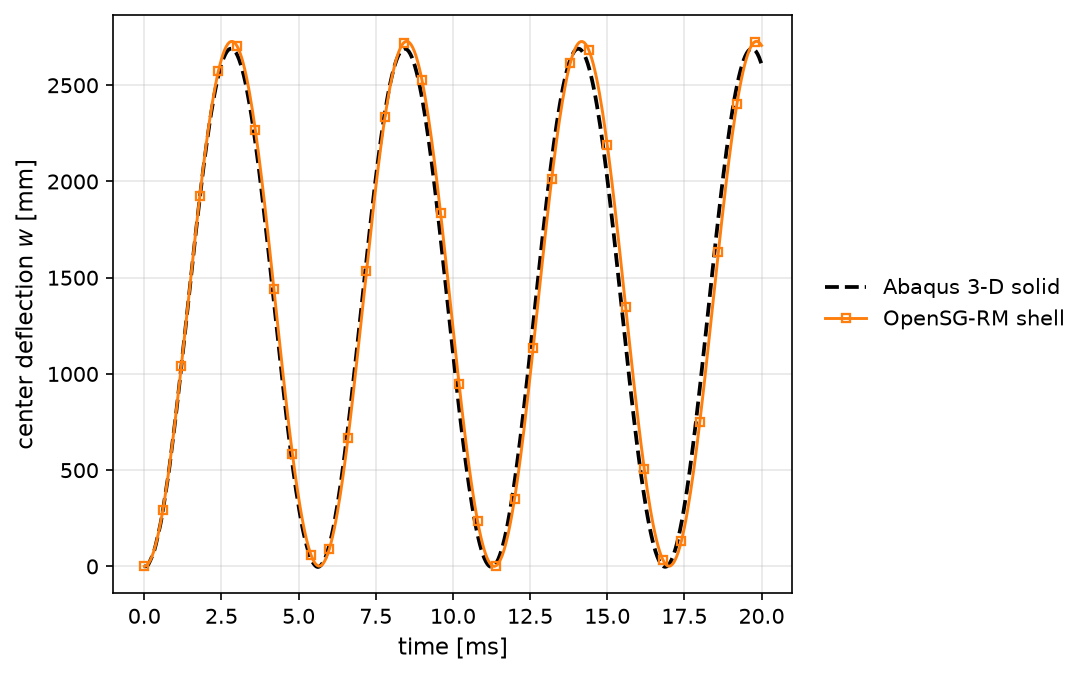
\includegraphics[width=.72\textwidth]{w_history_step.png}
\caption{Center deflection, step pulse: 3-D solid (benchmark) vs.\
OpenSG-RM vs.\ conventional Abaqus FSDT.}
\end{figure}
\begin{figure}[h!]\centering
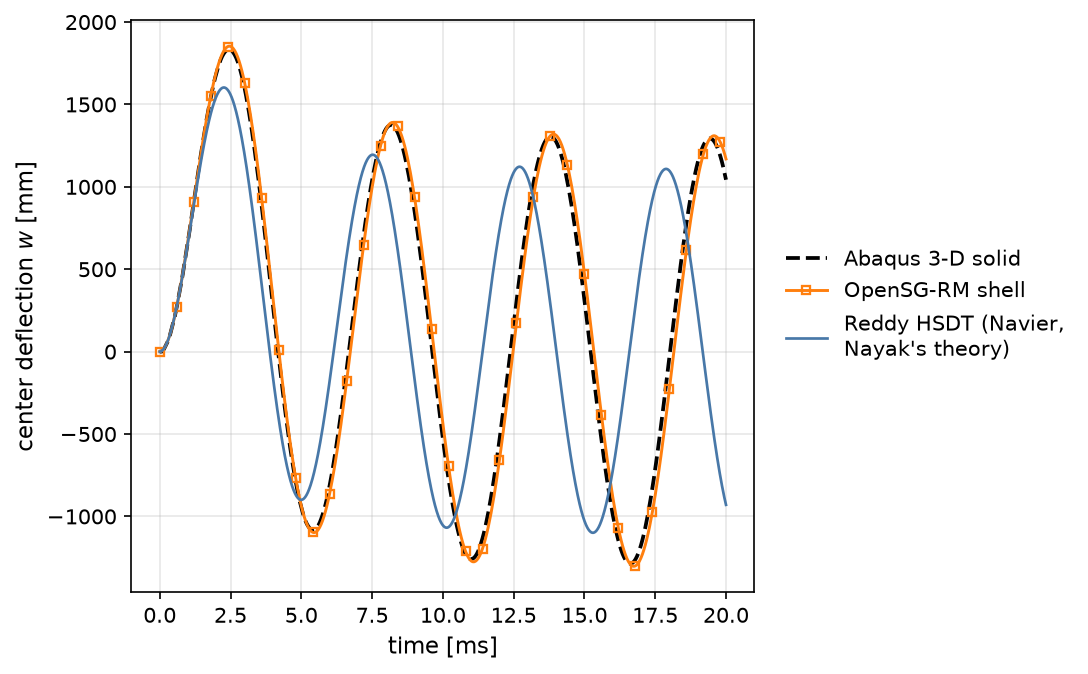
\includegraphics[width=.72\textwidth]{w_history_blast.png}
\caption{Center deflection, blast pulse.}
\end{figure}
\begin{figure}[h!]\centering
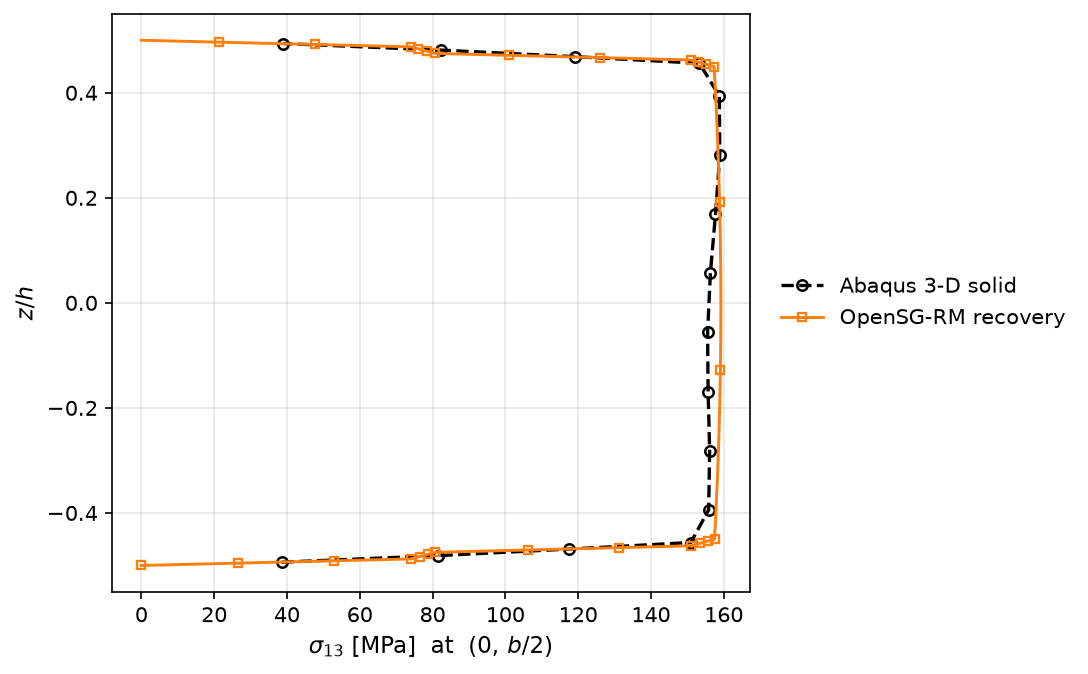
\includegraphics[width=.49\textwidth]{profile_s13_blast.png}
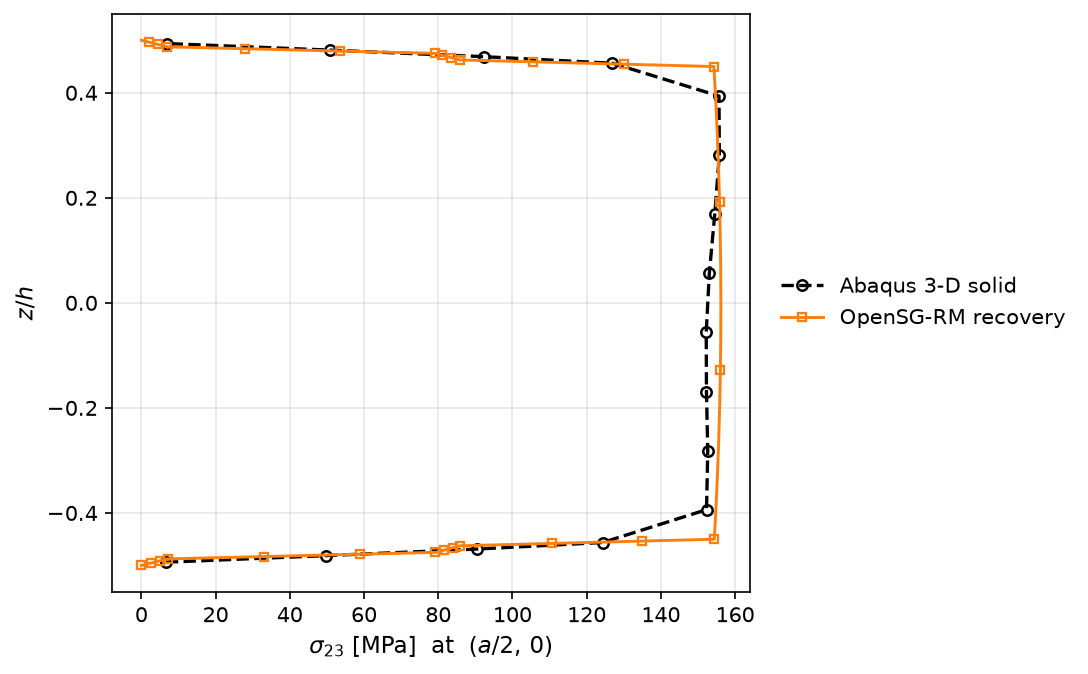
\includegraphics[width=.49\textwidth]{profile_s23_blast.png}\\
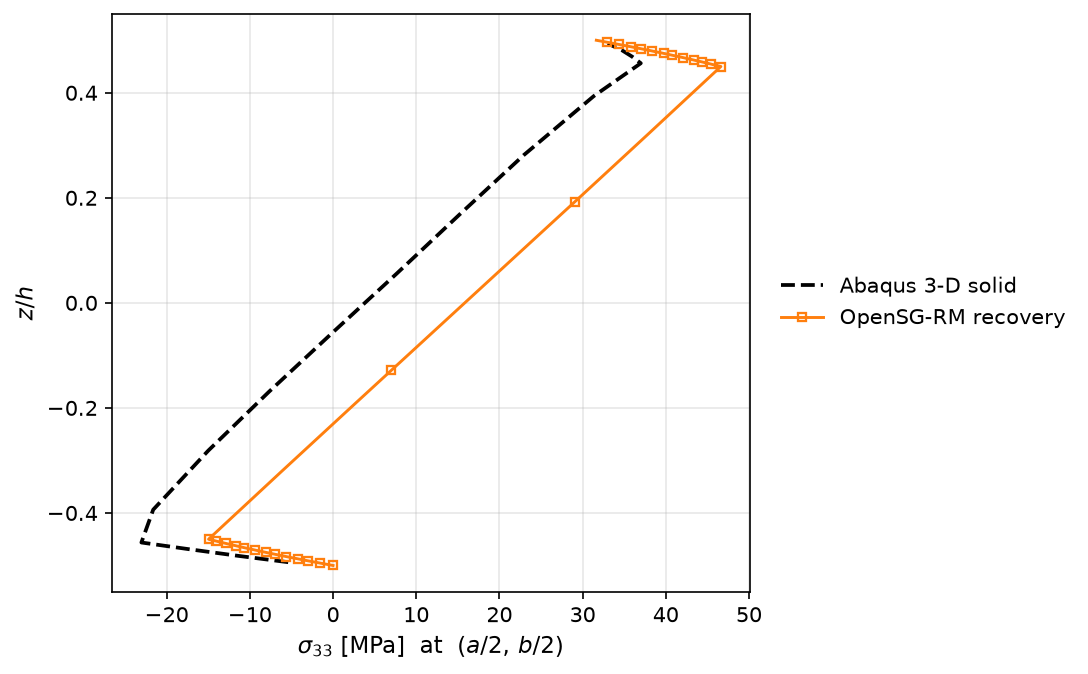
\includegraphics[width=.49\textwidth]{profile_s33_blast.png}
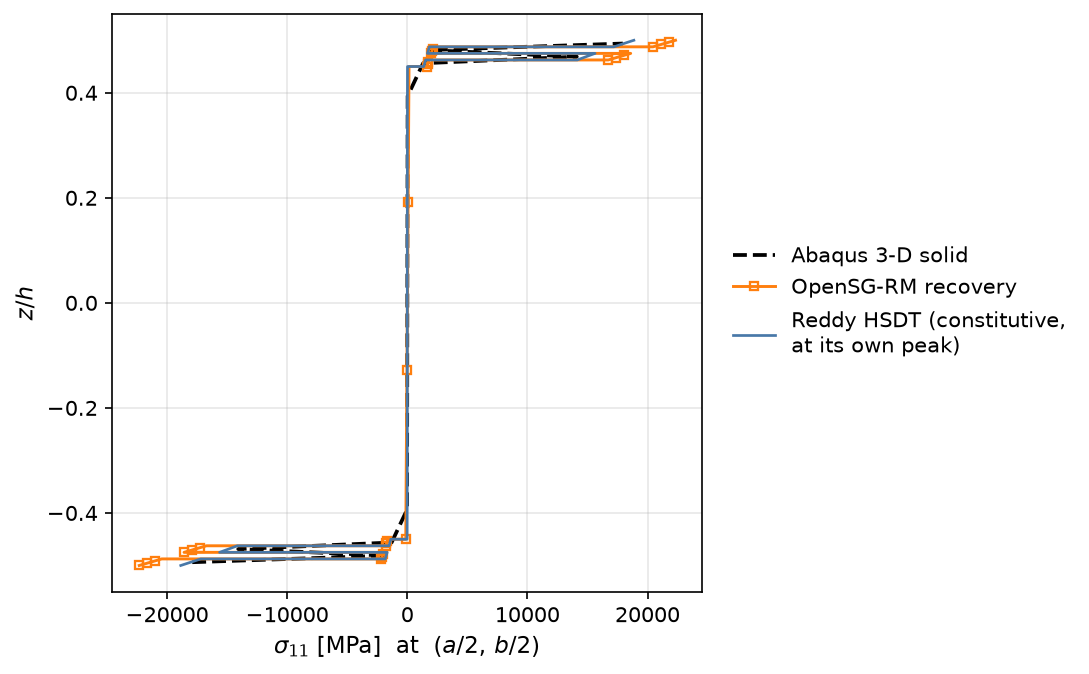
\includegraphics[width=.49\textwidth]{profile_s11_blast.png}
\caption{Through-thickness paths at the peak instant, blast pulse:
$\sigma_{13}(0,b/2)$, $\sigma_{23}(a/2,0)$, $\sigma_{33}$ and
$\sigma_{11}$ at the center --- recovery vs.\ solid.}
\end{figure}
\begin{figure}[h!]\centering
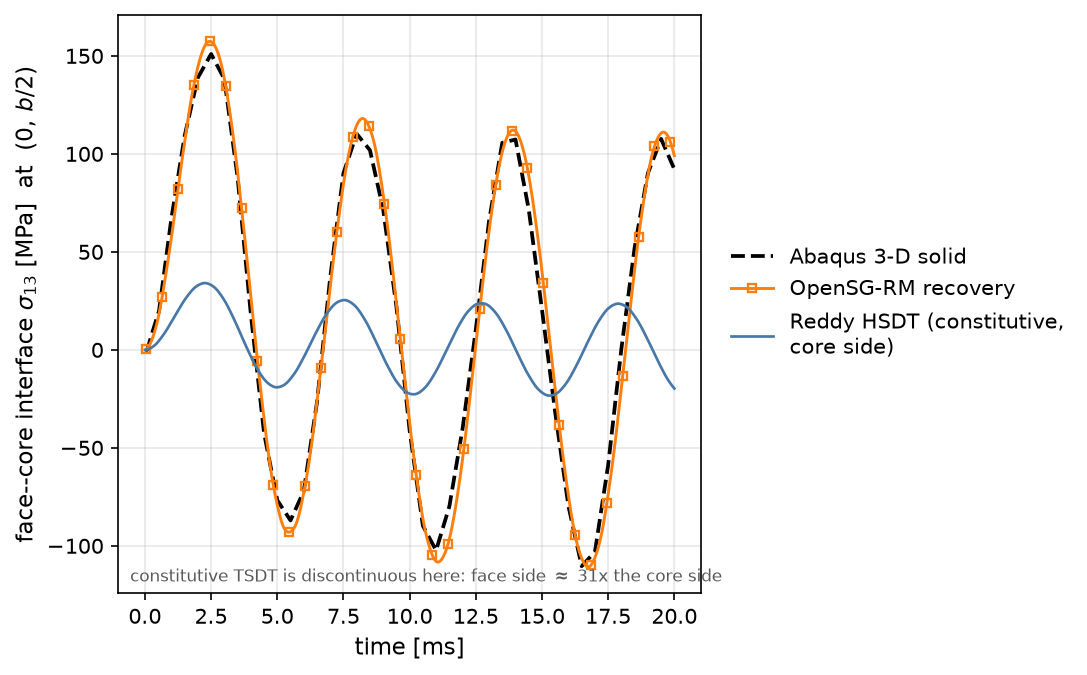
\includegraphics[width=.72\textwidth]{iface_s13_blast.png}
\caption{Face--core interface $\sigma_{13}$ history at $(0,b/2)$, blast
pulse: the design-driving debond quantity, available from the RM model at
every 50 $\mu$s.}
\end{figure}

\begin{center}\begin{tabular}{lcc}\toprule
peak center deflection & step & blast\\\midrule
Abaqus 3-D solid (benchmark) & 2.690 m & 1.834 m @ 2.451 ms\\
OpenSG-RM (S4 + MSG ABDG) & 2.728 m ($+1.4\,\%$) & 1.854 m ($+1.1\,\%$)
@ 2.450 ms\\
Abaqus FSDT (composite S4) & \multicolumn{2}{c}{see
\code{dyn\_step.dat}/\code{dyn\_blast.dat}}\\
\bottomrule\end{tabular}\end{center}

\paragraph{Findings.}
(i)~OpenSG-RM overlays the solid through 3.5 cycles (peak $+1.1$/$+1.4$\%,
frequency 178 Hz); (ii)~the conventional composite-shell FSDT --- the
route any commercial user would take --- inherits a face-dominated
transverse-shear stiffness and misses the sandwich dynamics (its curve and
peak error are in the deflection figures and the \code{dyn\_*.dat} files);
(iii)~the recovered $\sigma_{13}/\sigma_{23}$ reproduce the solid's core
plateau and face decays, and the interface $\sigma_{13}$ history tracks
the solid within $\sim$5\,\% at every 50 $\mu$s --- the solid affords that
quantity only at its dump instants; (iv)~cost: 37--39 s vs.\ 323--324 s
wallclock (8.7$\times$), 2646 vs.\ $\approx$22\,500 DOF.

\paragraph{Honest caveats.}
$\sigma_{33}$ through the soft core shows an $\approx$8--10 MPa
thickness-stretch offset mid-core (dynamic core compression --- 3-D
physics outside any 5-DOF plate kinematics); the first $\approx$0.3 ms is
genuinely 3-D (the pressure wave needs $\approx$0.15--0.2 ms to cross the
137 mm foam core); and Nayak's own sandwich figures (his Figs.~12--13)
could not be used quantitatively --- their period corresponds to a
face-dominated shear model and their amplitude scale is inconsistent with
the stated $q_0$ by orders of magnitude, so his \emph{tables} (Example 2)
served as the literature anchor instead.
\end{document}
